%mainfile: ../master.tex
\section{Models}
\label{sec:models}
Model is a term often used in both natural and social sciences. Unfortunately the term is perhaps not as well defined as it should be, and it will therefore be specified here. The approach here is based on Mario Bunge's definition of a model \cite{world_as_a_process}. According to his theory, a model consists of two parts:

\begin{itemize}
\item A general theory
\item A special description of an object or system
\end{itemize}

This perception is a very general way of thinking of models and often works very well with natural and, to some degree, social sciences where experiments and models are based on an overall theory and consists of objects and systems. In social sciences, though, it often happens that the general theory is vaguely defined or even non-existent and the purpose of the model is only to observe interactions and behaviour of the systems and their objects.
To extend Bunge's theory, models will here be defined as \enquote{a set of assumptions about a system} meaning everything we know about a system that we can observe or theorise about.
Generally there are two different types of models, static and dynamic models.


\subsection{Dynamic Models}
Dynamic models include some form of evolution, meaning that the system changes due to some changing factor. This is often time, but can also be things like energy, as is often the case in chemistry, the only important thing is that the factor changes. Nearly all systems in natural and social sciences are dynamic models.


\subsection{Static Models}
A static model is a snapshot of a given system with objects with non-changing states. These systems are often not very representative of reality, since nearly all physical systems change, but they can still be very useful to construct, since it can be much easier to collect information and understanding through a static model.


\section{Simulation}
We often need to create and analyse models when trying to get a better understanding of a given situation. For a portion of these models, an analytical approach can be used, where one can analyse the model via mathematical methods and calculate how static models will look and dynamic models evolve. This approach only works on a limited portion of the models, where the system and behaviour of objects are well known and can be described mathematically. As the models become more stochastic, purely mathematical analysis begins to fall short and simulations are often used to be able to create the models.

Formally, a simulation is \enquote{an imitation of a process through another process}~\cite{hegselmann1996modelling}. This is a very broad definition, since real world systems can be very different in their structure and the types of simulations also differ greatly. Generally one can distinguish between two different types of simulations, experimental and theoretical. An experimental simulation is where a real system is imitated by another real system, often smaller and/or simpler. For instance, when biologists simulate the creation of life on the back of crystals in their lab it is an experimental simulation. Theoretical simulations are simulations where a real system is imitated theoretically often on a computer or on paper. 

This project will focus on theoretical simulations. To further narrow the definition of a simulation used in this project, the focus will mainly be put on natural and social sciences where simulations are most often used. Within these sciences, real systems can still vary a lot, but they nearly always share the property that they change state over, what is often, but not necessarily, time. This is close to the definition of a dynamic model. In this respect simulations are close to a dynamic model. How this change is modelled can also vary and generally we often speak of two different paradigms; discrete and continuous simulations.

\subsection{Continuous Simulations}
Continuous simulations are simulations that are continuously evaluated. A continuous simulation is in many ways the most direct representation of reality, where actions and reactions happen based on each other and the environment they are in. It can be expressed as a differential equation. Just as with differential equations, a high precision is obtainable, but extracting results can prove to be cumbersome. But continuous simulations suffer in places were a granularity is hard to determine. Imagine, as an example, a simulation of light reflected in a solar system. If we were to conduct an experimental simulation of the light in a solar system, we could have a regular lightbulb represent the sun, and observe how different levels of power to the bulb changes the reflections in the model. But if we were to give a true accounting of the amount of photons a given star emits, the amount of calculations in a theoretical simulation would quickly grow out of reach for even the greatest supercomputer. This is a reason why continuous simulations can be problematic when implemented as a computer simulation.
\label{simulationchoise}


\subsection{Discrete Simulations}
Discrete simulations are simulations, where the state of the system is updated in discrete iterations. Observations in discrete simulations do not make sense during update but only before/after iterations. A discrete simulation tends to be more useful when certain abstractions can be made about the simulations. In the above mentioned example with the solar system, one might have observed not precisely when photons are emitted, but instead that every minute a certain number of photons are emitted on average. This could be modelled as a single emission of light every minute. This makes the calculation a lot simpler, but at the price of a loss of precision. Whenever a problem is discretisied, there will be a loss of detail.


\subsubsection{Granularity}

When creating a model for a theoretical simulation, there is usually a certain degree of information lost during modelling, due to either the process of isolation from the environment, or an omittance of details deemed insignificant. In the example of modelling the light reflected in a solar system, an example of isolation could be the omittance of light beeing emitted from other stars than the one residing in the solarsystem. In the same example, an omittance of details could be the interference of satellites orbiting a planet, effectively blocking some light from reaching the planet. Since the amount of light that is blocked by a satelite is miniscule in comparison, it could be deemed too insignificant to include this in the calculation, since it will likely not have any observable effect on the simulation. The choice of deciding the amount of details included, is known as choosing granularity.

Granularity, from the point of view of computer science, is a qualitative measure of the ratio of computation to communication. The granularities should be chosen, accordingly with the consideration of this ratio. Periods of computation are typically separated from periods of communication by synchronisation events.

One can say that \emph{fine-grain parallelism} is:

\begin{itemize}
\item Relatively small amounts of computational work is done between communication events
\item Low computation to communication ratio
\item Facilitates load balancing
\item Implies high communication overhead and less opportunity for performance enhancement
\item If granularity is too fine it is possible that the overhead required for communications and synchronisation between tasks takes longer than the computation.
\end{itemize}

and \emph{coarse-grain parallelism} is:

\begin{itemize}
\item Relatively large amounts of computational work is done between communication/synchronisation events
\item High computation to communication ratio
\item Implies more opportunity for performance increase
\item Harder to load balance efficiently
\end{itemize}

\subsubsection{Decomposition}
Decompositioning within computer science, is breaking a problem into discrete \enquote{chunks} of work that can be distributed as multiple tasks, for the computer to compute. In decompositioning the problem to multiple tasks, the designer of the solution can make use of two basic concepts: to partition the tasks in such a way that it can be parallelised by domain or functional decomposition.

\paragraph{Domain Decomposition} is distributing similar tasks of a problem among multiple different processors. \Cref{fig:dom} illustrates multiple similar tasks that can be parallelised, each working on their own domain of the problem set.

\begin{figure}[htbp]
\centering
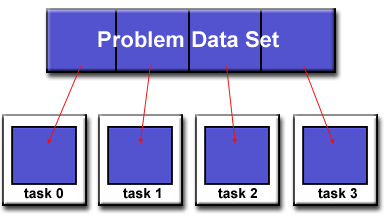
\includegraphics[width=0.7\textwidth]{Analysis/Supercomputing/domain_decomp.png}
\caption{Illustration of domain decompositioning. The problem data set is partitioned in chunks and then operated on by multiple tasks running in parallel. \cite{compLLNL}}\label{fig:dom}
\end{figure}

This is useful when working with data traversals of sets of data, if the operations of each iteration is independent of each other, the traversal can easily be split up into multiple parallel tasks.

\paragraph{Functional Decomposition} focuses on the operations performed rather than the data manipulated by the computation. Some tasks differ from others in that they manipulate different data of the problem domain. This is illustrated in \cref{fig:fun}.

\begin{figure}[htbp]
\centering
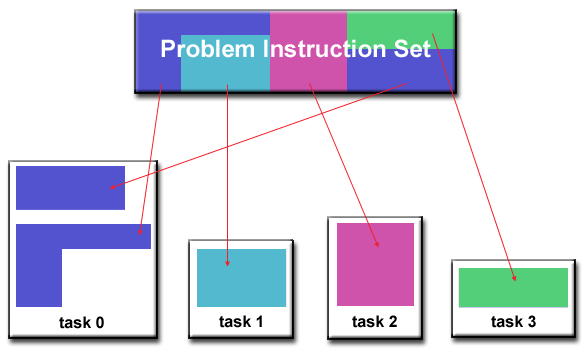
\includegraphics[width=0.7\textwidth]{Analysis/Supercomputing/functional_decomp.png}
\caption{Illustration of functional decompositioning in which each task performs operations on data in parallel. Each task has a predetermined operation to perform. \cite{compLLNL}}\label{fig:fun}
\end{figure}

The fact that we can decompose the problems into multiple independent tasks means that we make use of the performance provided in high performance computing (HPC) computers. The systems used in the field of HPC, relies on their many processor units to gain tremendous computational speed as opposed to the regular high throughput computing (HTC) computers, that ensures a reliable throughput instead.
